\section{技术方案}
\label{sec:technical-plan}
\subsection{系统总体架构}
FoodLens 将单张食物 RGB 图像映射为自然语言描述和结构化膳食记录。系统以两种自主描述模型建立可解释的对照，再将其中的视觉与序列模块迁移到食材生成和重量回归；预训练视觉语言模型提供独立的领域适配对照。图\ref{fig:fl-system}给出模块复用及评价关系。全部模型在推理时仅接收图像与固定任务指令，标签及含答案的元数据只用于监督和离线评价。
\begin{figure}[!ht]
\centering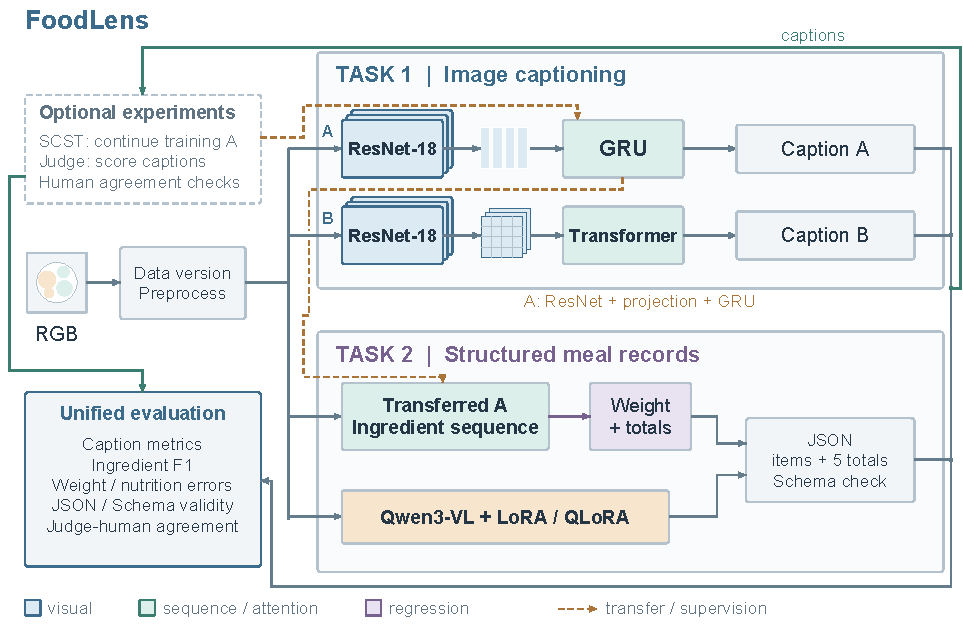
\includegraphics[width=\linewidth]{figures/architecture/figure06_system.pdf}
\caption{FoodLens 总体架构。实线表示数据流，虚线表示参数迁移或离线监督关系；两项任选实验复用描述模型及其输出。}
\label{fig:fl-system}
\end{figure}

共享数据层负责图文匹配、固定划分、文本编码和批处理，评价层接收按样本 ID 保存的预测文件，统一计算指标。任务一输出 Caption；任务二自主模型输出食材名称序列、对应重量与五维整餐数值，经确定性程序组装 JSON。Qwen3-VL 直接生成 JSON 文本，两条路线共用解析、Schema 校验与数值评价程序。该组织方式将模型能力与输出格式处理分开，便于追踪食材识别、定量估计和结构错误。

\subsection{食物图像描述生成模型设计}
\textbf{共享输入与文本表示。}两种自主模型均输入 $224\times224$ RGB 图像，使用 ImageNet 预训练 ResNet-18 的 \texttt{layer4} 输出 $F\in\mathbb{R}^{512\times7\times7}$，移除分类层\footnote{骨干输出位置与预处理依据 \href{https://docs.pytorch.org/vision/main/models/generated/torchvision.models.resnet18.html}{Torchvision ResNet-18 文档及其源码}。}。验证、测试采用短边缩放至 256 后中心裁剪，训练仅增加水平翻转，沿用预训练均值与标准差。两模型共享仅由训练 Caption 拟合的英文词级词表和规范化规则，保留标点，设置 \texttt{PAD/BOS/EOS/UNK}；最大生成长度初设为 64 Token，截断比例在训练前检查。以下维度和超参数均为起始配置，由验证集调整。


\textbf{模型 A：全局视觉条件的 GRU。}令 $v=\operatorname{GAP}(F)\in\mathbb{R}^{512}$，投影为 $z=\tanh(W_vv+b_v)\in\mathbb{R}^{256}$。采用 256 维词嵌入、单层 256 维 GRU，将 $z$ 同时作为初始隐藏状态和每步输入条件：
\begin{equation}
 h_0=z,\quad h_t=\operatorname{GRU}([E(y_{t-1});z],h_{t-1}),\quad
 p_\theta(y_t\mid y_{<t},I)=\operatorname{softmax}(W_oh_t+b_o).
 \label{eq:fl-gru}
\end{equation}
全局向量持续参与解码，降低长序列中视觉条件衰减的影响；输入拼接后的维度固定为 512，便于任务二直接复用 GRU 权重。

\begin{figure}[!ht]
\centering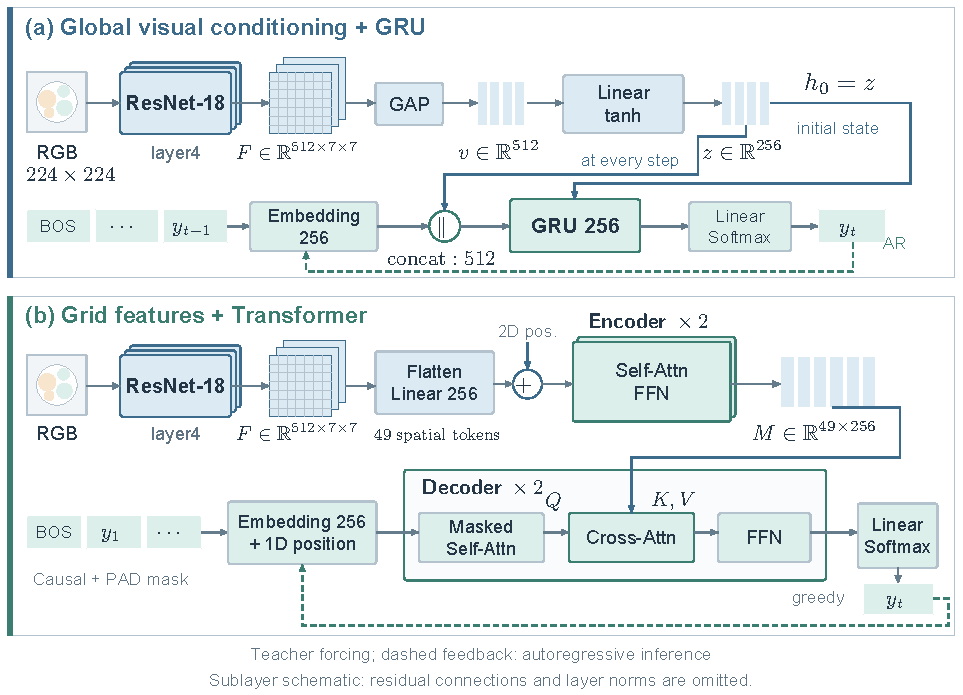
\includegraphics[width=\linewidth]{figures/architecture/figure07_caption.pdf}
\caption{任务一双模型内部结构。A 以全局条件驱动循环生成；B 保留 49 个空间位置，通过视觉自注意力及解码交叉注意力读取图像。训练输入为右移真实序列，推理输入为已生成前缀。}
\label{fig:fl-caption}
\end{figure}

\textbf{模型 B：网格视觉与 Transformer。}将 $F$ 展平为 $49\times512$，逐位置线性映射到 $d=256$，加上二维行列正弦位置编码，再由两层 Transformer Encoder 输出视觉记忆 $M\in\mathbb{R}^{49\times256}$。Decoder 初设两层、4 个注意力头、前馈维度 1024、Dropout 0.1，文本嵌入加一维位置编码。每层先执行因果自注意力，再以文本状态为 Query、$M$ 为 Key/Value 执行交叉注意力；每头维度为 64。固定大小网格无需视觉 Padding Mask，文本 Padding Mask 排除补齐位置；上三角因果掩码屏蔽未来 Token。该结构借鉴网格关系建模思路\cite{zeng2022s2}，不引入伪区域或多层网状连接。

\textbf{训练与解码。}Teacher Forcing 输入 $[\mathrm{BOS},y_1,\ldots,y_{T-1}]$，目标为 $[y_1,\ldots,y_{T-1},\mathrm{EOS}]$；交叉熵按全批非 PAD 目标数归一化，EOS 参与损失。先冻结骨干并保持 BatchNorm 为评价模式，训练投影与解码器；收敛后视验证结果以较小学习率解冻 \texttt{layer4}。主对照统一采用贪心生成，遇 EOS 或长度上限终止，束搜索仅作同协议补充。A 与 B 同时改变视觉表示和解码器，另设 B-Global：保留 B 的编码、解码配置，以投影全局向量形成单个视觉 Token，用一次轻量消融分析空间信息贡献。


\subsection{结构化膳食记录生成}
\subsubsection{自主混合预测架构与参数迁移}
任务二采用\textbf{共享视觉编码、食材序列生成、边界位置重量回归和整餐数值回归}的多任务结构，如图\ref{fig:fl-hybrid}。从任务一 A 的最优监督 Checkpoint 迁移 ResNet-18、$W_v,b_v$ 和 GRU；新增重量与营养回归头。食材序列使用与任务一相同的词级切分规则，在原词表后追加任务二训练集词语和边界 Token \texttt{SEP}，按 Token 字符串复制已有嵌入和输出层行，新行随机初始化。保留原词表 ID，验证集和测试集不参与扩词。这样既保留语言参数，也明确迁移范围。

\begin{figure}[!t]
\centering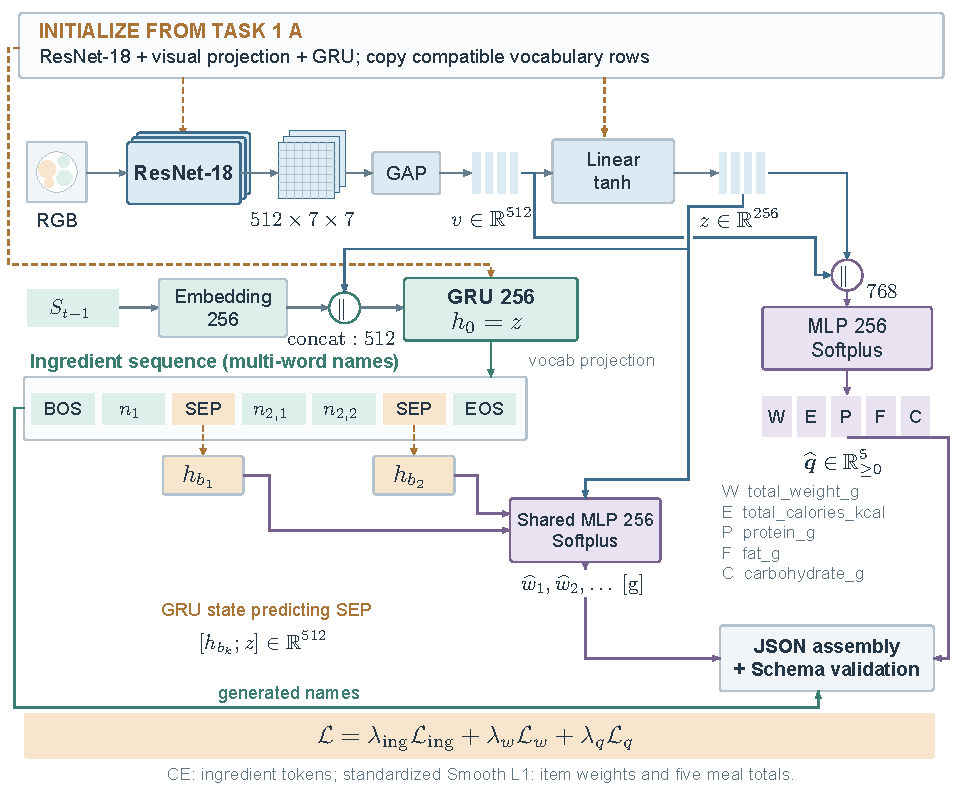
\includegraphics[width=\linewidth]{figures/architecture/figure08_hybrid.pdf}
\caption{任务二自主混合架构。第 $k$ 个 SEP 的预测状态 $h_{b_k}$ 来自产生该 SEP logits 的 GRU 隐藏状态，虚线按边界位置选取；整餐五维数值由独立分支预测。虚线为迁移或监督，推理时沿实线动态组装记录。}
\label{fig:fl-hybrid}
\end{figure}

\textbf{食材列表序列化。}名称先执行 Unicode 规范化、小写化与空白合并，不做基于测试标签的同义词扩展。同一记录中相同规范化名称合并并累加重量，再按名称字典序排序，得到 $K$ 项 $\{(n_k,w_k)\}_{k=1}^K$。监督序列为
\begin{equation}
 S=[\mathrm{BOS},\operatorname{tok}(n_1),\mathrm{SEP},\ldots,
 \operatorname{tok}(n_K),\mathrm{SEP},\mathrm{EOS}].
 \label{eq:fl-items}
\end{equation}
每个名称可占多个词，SEP 标识完整名称结束，排序规则减少同一集合多种排列带来的监督歧义。食材分支仍按式\eqref{eq:fl-gru}逐词生成；不以训练食材全名白名单约束解码，以允许已知词组成新名称。全新词映射至 UNK，含 UNK 的项记为识别失败；即便后续改用子词编码，开放名称的可表示性也需与视觉识别准确性分别验证。


\subsubsection{食材边界对齐与多任务训练}
\textbf{逐食材重量。}定义 $b_k$ 为目标 SEP 在预测序列中的时间步，$h_{b_k}$ 表示\emph{产生该 SEP 的 logits 所用状态}。Teacher Forcing 时该状态已读取完整的第 $k$ 个真实名称；批处理额外保存 $b_k$、$w_k$ 与有效项掩码，按位置 Gather 隐藏状态，不对 PAD 或普通词位置计算重量损失。推理每产生一个 SEP，便从同一位置提取状态并回归一项重量，输出项数由生成边界动态决定：
\begin{equation}
 \widehat w_k=\operatorname{softplus}(f_w([h_{b_k};z])),\qquad
 \widehat{\boldsymbol q}=\operatorname{softplus}(f_q([v;z]))\in\mathbb{R}_{\geq0}^{5}.
 \label{eq:fl-regression}
\end{equation}
两个 $f$ 为独立的两层 MLP，隐藏维度初设为 256。$\boldsymbol q$ 按固定顺序表示总重量、总热量、蛋白质、脂肪和碳水化合物，分别以 g、kcal、g、g、g 为单位。输出经 Softplus 保证非负，整餐头不依赖生成的食材前缀，避免名称错误直接阻断全部数值输出。

\textbf{尺度与联合目标。}以训练集估计逐项重量及每个整餐字段的均值 $\mu_j$、标准差 $s_j$，将 $s_j$ 下限设为 $10^{-6}$。模型先输出原单位非负值，再以 $\mathcal N_j(a)=(a-\mu_j)/s_j$ 同时变换预测和标签，计算尺度一致的 Smooth L1（阈值 1）：
\begin{align}
 \mathcal L_{\rm ing}&=-\frac{1}{N_{\rm tok}}\sum_{i,t}m_{it}
       \log p_\theta(S_{it}\mid S_{i,<t},I_i),\notag\\
 \mathcal L_w&=\frac{1}{N_{\rm item}}\sum_{i,k}a_{ik}
   \ell\bigl(\mathcal N_w(\widehat w_{ik}),\mathcal N_w(w_{ik})\bigr),\notag\\
 \mathcal L_q&=\frac{1}{5B}\sum_{i=1}^{B}\sum_{j=1}^{5}
   \ell\bigl(\mathcal N_j(\widehat q_{ij}),\mathcal N_j(q_{ij})\bigr),\notag\\
 \mathcal L&=\lambda_{\rm ing}\mathcal L_{\rm ing}+\lambda_w\mathcal L_w+
       \lambda_q\mathcal L_q.\label{eq:fl-joint}
\end{align}
其中 $m_{it}$ 排除 PAD，$a_{ik}$ 标识真实食材，$N_{\rm tok}$、$N_{\rm item}$ 为相应有效数，$B$ 为批大小；无有效项时重量损失置零。三个权重先取 1，观察各损失及梯度量级，仅在验证集上小范围调整。训练先冻结视觉骨干联合学习新任务，再按需解冻末级视觉层。重量监督使用真实名称条件，最终评价使用自由生成结果，二者差异作为误差传播分析的一部分。

\textbf{JSON 组装。}推理限制首项非空、SEP 前至少有一个名称词、EOS 只出现在列表边界；达到长度或项数上限时丢弃未闭合末项并记录截断。空名、UNK 和非有限重量进入失败记录；有效重复名称按名称合并、重量求和。输出根对象含 \texttt{items} 及五个数值字段，项对象仅含 \texttt{name}、\texttt{weight\_g}；验证字段集合、非空字符串、数值类型、有限性与非负性，拒绝布尔值和额外字段。组装时统一保留一位小数，数值评价使用同一交付值。依据已有审计，食材重量之和与整餐重量分别学习，\textbf{不设置二者相等的约束}。原始输出、清理日志与最终 JSON 同时留存，便于区分生成和后处理收益。


\subsubsection{Qwen3-VL 的领域参数高效适配}
预训练路线采用 \textbf{Qwen3-VL-4B-Instruct}，使用其官方 Processor 和 Chat Template 组织图像与对话\footnote{输入格式及微调入口参考 \href{https://huggingface.co/Qwen/Qwen3-VL-4B-Instruct}{官方模型卡}与 \href{https://github.com/QwenLM/Qwen3-VL}{Qwen3-VL 官方仓库}，实施时固定版本与模型 revision。}。每个样本的 user 消息包含 RGB 图像、固定膳食记录指令、字段与单位说明；assistant 消息为统一序列化的目标 JSON。仅 assistant 目标及其结束标记参与自回归交叉熵，系统提示、user 内容、图像占位和 PAD 的标签置为忽略值。训练前在单样本上逐段检查掩码，保留多模态控制 Token，序列超限时先控制图像 Token 与长度，不截断监督 JSON。

\begin{figure}[!t]
\centering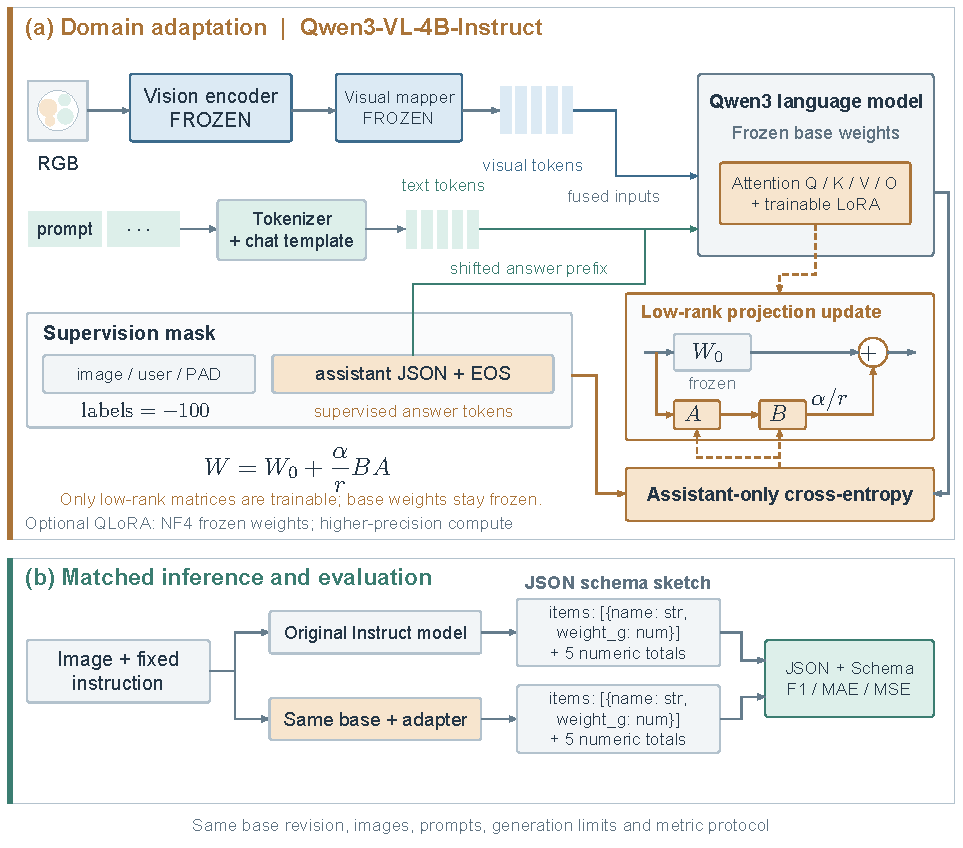
\includegraphics[width=\linewidth]{figures/architecture/figure09_qwen.pdf}
\caption{Qwen3-VL 领域适配流程。仅目标回答参与监督；同一基础模型在相同输入、生成和评价协议下比较适配前后差异。量化为可选存储策略，视觉部分初始冻结。}
\label{fig:fl-qwen}
\end{figure}

\textbf{适配与资源控制。}初始冻结视觉编码器、视觉语言映射及语言基础权重，在语言模型注意力的 Q/K/V/O 线性投影中注入 LoRA\cite{hu2022lora}，初设 $r=8$、$\alpha=16$、Dropout 0.05。依据模型实际模块路径限定注入范围，并输出可训练参数清单，避免同名视觉层被误选。先做小批量显存试跑：常规 BF16 LoRA 能容纳目标序列则优先采用；空间不足且算子兼容时，采用 NF4 4-bit、双重量化的 QLoRA\cite{dettmers2023qlora}，冻结量化权重，以 BF16 或硬件支持的计算精度训练适配器。配合梯度累积、梯度检查点和图像分辨率上限控制开销，保持任务目标不变。

主实验比较同一 4B revision 的原始 Instruct、领域微调版本及自主混合模型；若 24 GB 单卡环境无法稳定运行，成对切换到同一 2B 基础模型重新比较，单独报告规模。图像预处理、固定指令、最大输出长度及贪心解码在适配前后保持一致。生成文本先严格解析再校验 Schema，主指标不做提示重试或内容修复；失败样本进入全样本统计。保存原始字符串、错误类型与成功解析值；如附加格式修复实验，单列其结果。模型、适配器、Processor、量化配置和解码配置共同构成可复现的推理版本。


\subsection{训练优化与多模态评价}
\subsubsection{从监督训练衔接 SCST}
任选优化优先用于任务一模型 A。先按验证集 CIDEr-D 选定交叉熵训练 Checkpoint，再复制该权重进入低学习率 SCST 阶段\cite{rennie2017scst}。对同一训练图像，生成采样序列 $y^s\sim p_\theta$ 和贪心序列 $y^g$，使用训练参考描述计算 CIDEr-D 奖励 $r$：
\begin{equation}
 \mathcal L_{\rm SCST}=-\operatorname{stopgrad}\bigl[r(y^s)-r(y^g)\bigr]
   \sum_{t\leq T_s}\log p_\theta(y^s_t\mid y^s_{<t},I).
 \label{eq:fl-scst}
\end{equation}
EOS 参与概率和，EOS 后的 PAD 不参与；采样与贪心分支采用一致的模型模式和最大长度，基线与奖励不反向传播。CIDEr-D 文档频率仅由训练参考预计算并固定，避免随小批次改变奖励标尺。训练初期可使用 $\mathcal L_{\rm mix}=(1-\eta)\mathcal L_{\rm CE}+\eta\mathcal L_{\rm SCST}$，$\eta$ 初设 0.5，再由验证稳定性决定是否调整。

最小交付为同一 A 模型监督训练前后两个版本、完全一致的测试解码与四项文本指标，并保存逐样本奖励及典型描述。除 CIDEr-D 外，同时检查 BLEU-4、METEOR、ROUGE-L 和食材幻觉，分析优化目标提升是否伴随细节与可读性的改变。若预算允许，增加相同步数继续交叉熵的对照，以区分额外训练与奖励优化的作用。

\subsubsection{固定协议的 VLM-as-Judge 与人评对照}
评价借鉴 CLIPScore 的图文相容性\cite{hessel2021clipscore}以及 FLEUR、EXPERT 的视觉条件评分和解释组织\cite{lee2024fleur,kim2025expert}。使用冻结的原始 Instruct VLM 作 Judge，独立于领域微调权重；输入仅为图像、候选 Caption 和固定评分标准，隐藏模型名称及参考描述。四维均采用 1--5 分，语义正确性检查主要菜品与关系，细节覆盖检查可见属性，事实可靠性以高分表示少幻觉与错误食材，语言流畅度检查语法及自然程度。每维同时输出一句图像证据，固定模型 revision、提示模板、温度 0 与解析规则，解析失败率另行报告。

初始从测试集固定抽取约 60 张图像，覆盖菜品类别、长短描述与困难样本；在查看模型结果前锁定样本 ID。比较 A、B、A+SCST 的同图输出，以随机顺序、匿名方式交给两名组员独立评分，少量分歧样本由第三名组员讨论裁定。用 Spearman 相关衡量 Judge、传统指标与人工均分的一致性，按图像进行 Bootstrap 给出区间，另报两名人评的加权 Cohen $\kappa$。人工样本较少时以维度趋势和错误案例为主；Judge 使用固定评分协议，不训练专门评价模型。记录同系列模型可能带来的偏好，并保留与人评不一致的原始解释供复核。


\FloatBarrier
\subsection{数据处理与实验设计}
\textbf{Food-500 Cap 的可靠映射与划分。}官方说明将数据分为 19,760 条训练和 4,940 条测试图文对\cite{ma2023food}；本地标注文件实际为 19,880 和 4,940 条，须记录这一版本差异。本地图片来自社区镜像，先以官方 \texttt{filename}、类别与镜像索引建立显式映射，以官方 Caption 为文本依据；无法唯一确认的映射排除并记录，图像解码失败单列。复用已有审计结论处理少量缺失、映射差异及重复图像，固定文件 SHA-256、数据源 revision、排除原因和最终样本清单，不凭行号直接拼接图文。

对于跨官方训练/测试的相同图像组，测试归属优先，移除训练侧副本；同一测试重复组仅保留稳定排序后的一个代表。近重复组复核后采用相同策略。再按重复组从剩余官方训练集划出约 10\% 验证样本，以类别分层尽量保持分布，种子设为 42；组内样本不跨划分。清洗后的计数以 manifest 为准，与原始数量分别报告。词表、长度统计及 SCST 奖励统计均仅从最终训练集拟合。

\textbf{结构化数据与输入隔离。}本地 \texttt{nutrition5k-student-v1} 包含 Train 2,338、Validation 414、Test 506，共 3,258 条，保留学校原始划分。数据加载器将 \texttt{image} 与 \texttt{target} 分开返回，推理接口只允许图像及固定指令，禁止传入 \texttt{target\_text} 和含答案的 \texttt{metadata}。已有审计发现可变项数、训练未见食材、总量不一致及少量疑似同餐跨划分，故主结果沿用原划分，并在已标记疑似组上附分层敏感性分析。所有阈值、规范化映射与模型选择均在训练/验证阶段确定，测试集仅用于冻结方案后的最终评价。

\begin{table}[!htbp]
\caption{统一评价协议与失败样本计入方式}
\label{tab:fl-metrics}\centering\small
\setlength{\tabcolsep}{4pt}\renewcommand{\arraystretch}{1.15}
\begin{tabularx}{\linewidth}{@{}P{2.35cm}YP{4.0cm}@{}}\toprule
\textbf{对象} & \textbf{主要指标与统计单位} & \textbf{协议要点}\\\midrule
Caption & BLEU-4、METEOR、ROUGE-L、CIDEr-D；语料级得分 & 同一 Tokenizer、单参考、实现版本与缩放单位\\
食材名称 & Micro F1 为主，Macro F1 为辅；见过/未见名称分层 & 规范化全名精确匹配，预测无效项计 FP\\
食材重量 & 匹配项 MAE/MSE；全名称并集 MAE/MSE & 漏检与多检按另一侧重量为零计入\\
整餐五维 & 各字段原单位 MAE、MSE，逐字段报告 & 解析失败采用预先规定的零预测计误差\\
输出结构 & JSON 语法合法率、Schema 有效率 & 分母均为全部样本；额外报告截断/失败率\\\bottomrule
\end{tabularx}
\end{table}

\textbf{名称匹配与重量误差。}真实和预测项采用同一名称规范化及重复项合并。按全名精确匹配，不用重量进行匹配，避免利用数值标签挑选最有利配对。令 $U_i$ 为两侧名称并集，缺失侧重量置零，定义
\begin{equation}
 E_{\rm union}^{(p)}=\frac{\sum_i\sum_{n\in U_i}|\widehat w_i(n)-w_i(n)|^p}
 {\sum_i|U_i|},\qquad p=1,2.\label{eq:fl-union}
\end{equation}


式\eqref{eq:fl-union}分别为并集 MAE 和 MSE，同时惩罚漏检和多检。匹配项误差单列，并给出匹配覆盖率；无匹配项记为不可计算，不记为零误差。非法名称项保留为互不匹配的预测项，计 FP 及其可读重量误差；完全无法解析的输出视作空食材集合、整餐零预测，仍保留在全样本分母中。另报有效输出子集误差与覆盖率，解释零预测约定的影响。对未见名称分别统计全名与组成词是否在训练集出现。辅助文本指标可用于规范化食材序列或 JSON，但不替代名称、重量及结构评价。

\begin{table}[!htbp]
\caption{按实施优先级组织的最小实验矩阵}
\label{tab:fl-experiments}\centering\small
\setlength{\tabcolsep}{4pt}\renewcommand{\arraystretch}{1.13}
\begin{tabularx}{\linewidth}{@{}P{1.55cm}P{4.6cm}Y@{}}\toprule
\textbf{层次} & \textbf{实验组} & \textbf{主要问题}\\\midrule
必选一 & A、B；共享划分与贪心解码 & 全局循环与网格注意力两条路线的总体差异\\
必选二 & 自主混合；同规模原始/微调 Qwen & 食材、定量与结构质量的领域适配收益\\
轻量消融 & B-Global；混合模型仅视觉迁移 vs. 视觉+GRU 迁移 & 空间信息贡献、序列迁移是否有效\\
任选 & A 的 CE vs. SCST；Judge 与双人人评 & 奖励优化收益、评分一致性与幻觉变化\\\bottomrule
\end{tabularx}
\end{table}

主对照固定清洗版本、训练预算与选择规则，记录参数量、可训练参数、单图推理耗时和实际显存。自主模型在预算允许时使用三个种子，报告均值与标准差；VLM 优先完成一个固定种子的配对适配实验，明确重复次数。任务一按验证 CIDEr-D 选模型；任务二按验证 Micro F1 选模型，接近时比较五维标准化 MAE，再比较有效率，规则在测试前固定。误差分析覆盖可见/隐含食材、长列表、未见名称、大份量、疑似同餐样本及重度质量不守恒样本，不将这些标记作为推理输入。

\subsection{工程实现与可行性分析}
采用 PyTorch 与 Torchvision，自主编写条件生成、掩码、损失、解码、边界对齐与记录组装；Transformer 可复用标准层，VLM 使用 Transformers、PEFT 和兼容的量化后端。工程拆分为数据与 manifest、Tokenizer、视觉骨干、序列解码器、回归头、训练器、解码器、Schema 与指标模块。训练接口接收图像及监督，返回分项损失；推理接口只接收图像和配置，返回逐样本预测及状态。先用 CPU 小样本验证尺寸、因果掩码、边界 Gather、梯度流、非负输出与 JSON 往返，再进入 GPU 训练。

配置统一保存种子、数据哈希、词表、数值统计、模型维度和生成参数；Checkpoint 保存模型、优化器、调度器、随机数状态及版本信息。自主模型初设 AdamW、学习率 $3\times10^{-4}$、梯度裁剪 1.0；视觉层解冻后使用主学习率的十分之一，采用验证早停。总算力预算约 300 元，计划单卡 24 GB，先完成两项必选任务及同规模微调对照，再复用已有模型开展任选实验。GPU 型号、LoRA/QLoRA 最终配置、批量与步数由小样本试跑和预算共同确定，不预设训练时长或峰值显存。

主要风险集中在 RGB 份量歧义、小数据过拟合、食材序列训练与自由生成的差异，以及多模态量化兼容性。通过冻结骨干、验证早停、全样本指标和输出追踪控制风险；主混合分支若难以收敛，回退到共享 ResNet 的多标签食材预测加数值回归，并保留回退原因。优先交付可复现的完整推理与评价链路，再增加网格交叉注意力等局部增强。上述设计为待实施方案，模型效果及资源数据均由后续实验给出。
